\section{Methodology}
\label{sec:methodology}

\begin{figure}[t]
  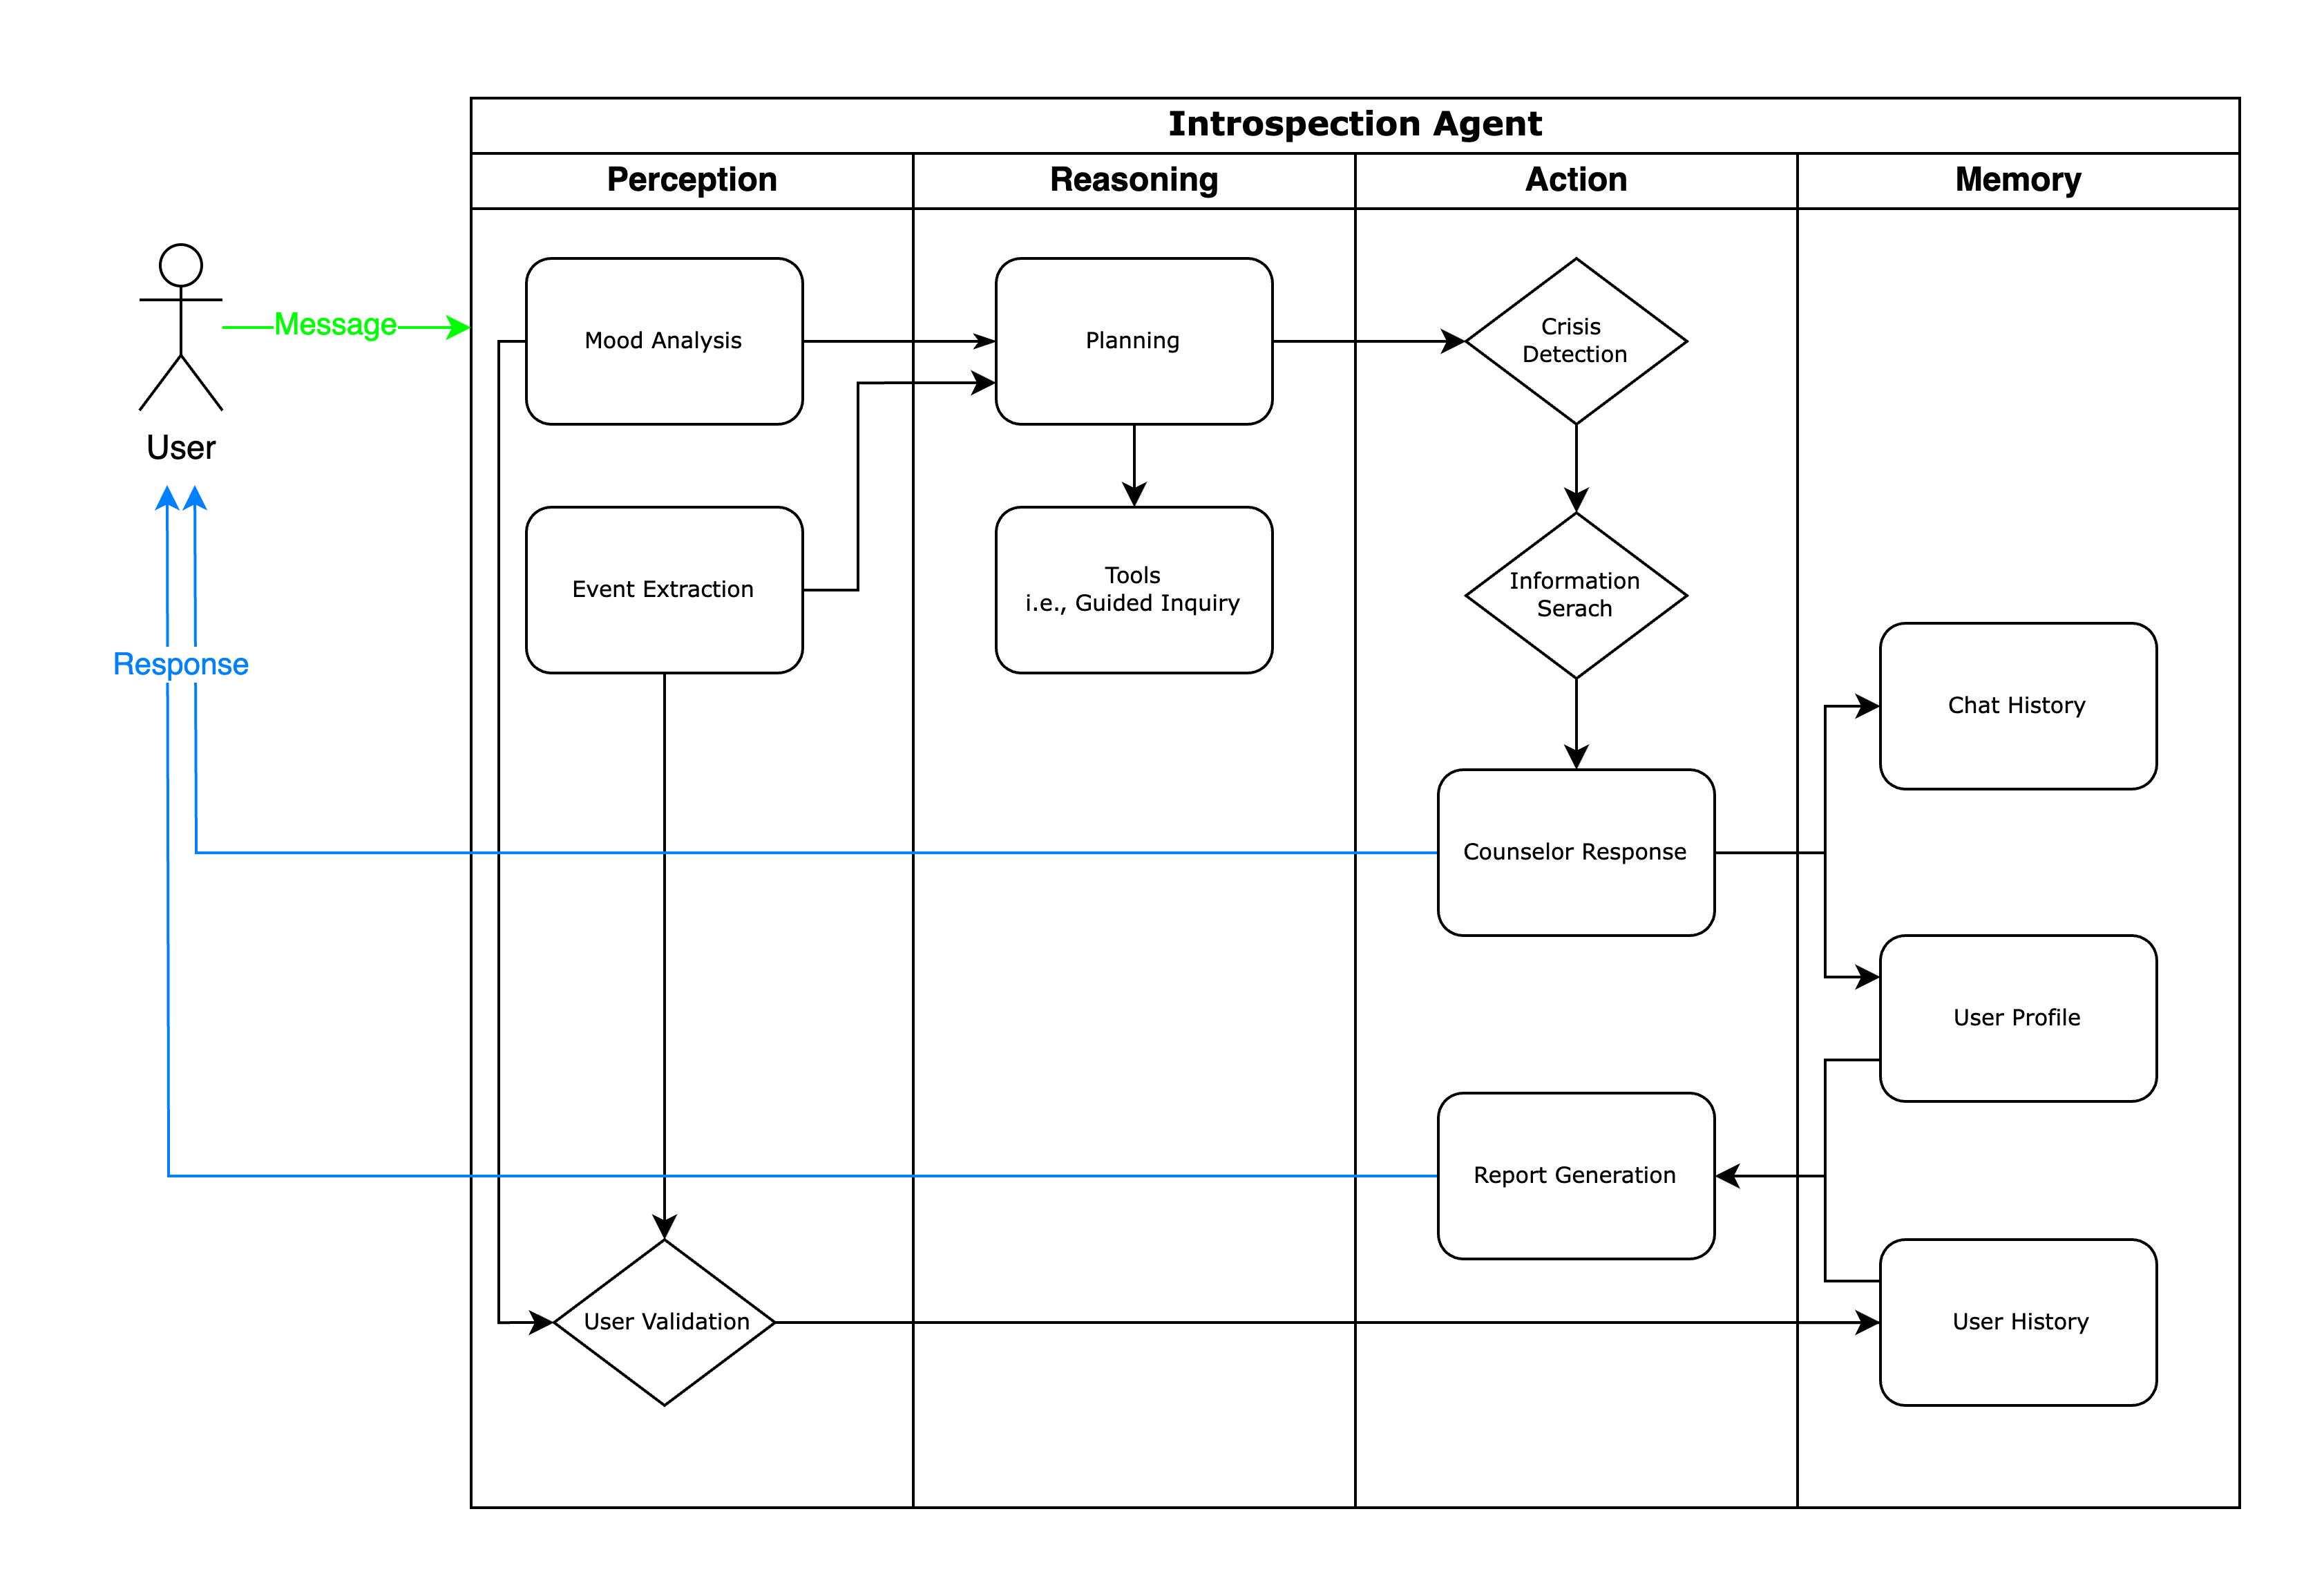
\includegraphics[width=\columnwidth]{figs/introspection-agent.png}
  \caption{An overview of introspection agent.}
  \label{fig:introspection-agent}
\end{figure}

In this section, we first provide an overview of how the Introspection Agent operates, followed by a detailed discussion of its main components.

As illustrated in Figure~\ref{fig:introspection-agent}, the agent is organized into four key modules: \textbf{Perception}, \textbf{Reasoning}, \textbf{Action}, and \textbf{Memory}. Upon receiving user input, the system initially performs \textit{Mood Analysis} and \textit{Event Extraction} to interpret the user's emotional state and contextual information. The \textbf{Reasoning} module then engages in \textit{Planning} and leverages tools such as \textit{Guided Inquiry} to process the user's request. If a potential crisis is detected (\textit{Crisis Detection}), the system immediately enters a crisis intervention phase and provides a psychological help hotline. If a search intent is identified, the system conducts an \textit{Information Search} before generating a \textit{Counselor Response}. 

Throughout this process, all interactions are systematically logged in the \textit{Chat History}, \textit{User Profile}, and \textit{User History}, enabling continuous learning and personalized user experiences.

\subsection{Perception}

\subsubsection{Mood}

TODO@Wang Xueyao  

The mood analysis feature represents a sophisticated integration of large language model (LLM) capabilities with clinical psychology principles, specifically designed to provide continuous, contextually-aware emotional evaluation.

\paragraph{Data Structure}

The analytical foundation leverages meticulously engineered prompts that instruct the LLM to function as an emotion analysis expert, ensuring consistent and clinically-relevant outputs. This prompt engineering approach directs the model to analyze conversational data and return a structured JSON schema encompassing four fundamental dimensions that align with established psychological frameworks, particularly Cognitive Behavioral Therapy (CBT) principles.

\begin{itemize}
\item \textbf{Mood Intensity:} A normalized scalar value ranging from 0 to 10, providing a quantitative measure of emotional arousal. This continuous scale enables nuanced tracking of emotional fluctuations and facilitates longitudinal analysis of affective patterns.

scheme

\item \textbf{Mood Category:} A discrete emotional classification drawn from a comprehensive taxonomy of psychological states (e.g., Sad,'' Anxious,'' ``Excited''). This categorical approach aligns with established psychological frameworks while maintaining sufficient granularity for clinical relevance.

\item \textbf{Thinking:} A verbatim quote or paraphrased representation of the user's potential inner monologue or cognitive appraisals (e.g., ``I am a failure''). This dimension serves as a critical component for identifying cognitive distortions, a fundamental concept in Cognitive Behavioral Therapy (CBT), enabling therapeutic interventions targeting maladaptive thought patterns.

\item \textbf{Scene:} The contextual trigger or situational antecedent associated with the emotional response (e.g., ``Seeing a friend's post on social media''). This contextual grounding facilitates the identification of environmental triggers and supports the development of situation-specific coping strategies.
\end{itemize}

This multi-faceted analytical framework transcends traditional sentiment analysis by providing a comprehensive psychological profile that captures not merely the valence and arousal of emotions, but also their cognitive and contextual underpinnings.

\paragraph{Technical Implementation Architecture}

\begin{enumerate}
\item \textbf{MoodService }\\
The system implements a dedicated LLM-based analytical service, designated as the MoodService, which operates through a discrete LLM instance (specifically, Qwen3-32B) to ensure computational independence from primary conversational functions. This service is governed by meticulously engineered prompts, which constrains model outputs to conform to predefined analytical specifications while maintaining focus on comprehensive psychological evaluation. In addition, the architectural segregation  ensures that intensive mood analysis computations do not compromise real-time conversational responsiveness, thereby preserving user experience integrity.

    \item \textbf{Contextual Batch Processing}\\
The system employs a sliding window methodology for contextual message processing, systematically extracting and analyzing the seven most recent user messages subsequent to each conversational interaction. This temporal windowing approach facilitates the incorporation of conversational context essential for accurate emotional state detection while enabling the identification of emotional progression patterns rather than discrete affective snapshots. 

\item \textbf{Feedback Integration}

To optimize user experience and prevent cognitive overload, the system implements an intelligent refresh algorithm for mood data updates that operates under dual criteria: when mood intensity exceeds 0.8 on the normalized scale, indicating emotionally significant states, and when the detected mood category differs from the previous assessment, preventing redundant notifications. This approach ensures users receive alerts only for meaningful emotional transitions, reducing notification fatigue while maintaining clinical relevance and therapeutic value.

Upon navigation to the mood analysis interface, the system presents automatically generated emotional assessments in a structured, visually accessible format with mood intensity, category, cognitive content, and situational context displayed in an initially read-only state, allowing users to inspect assessments without inadvertent modification. The system incorporates feedback mechanisms through editing functionality that enable users to correct misidentified emotional states or contextual elements. All user interactions include real-time UI feedback through toast notifications and visual state indicators, ensuring transparency and maintaining engagement throughout the assessment process.

\item \textbf{Data Management}

The system's backend architecture supports comprehensive data management through structured data transmission using RESTful API endpoints with standardized JSON schemas, ensuring data integrity and interoperability across system components. Each mood record incorporates session identifiers and temporal metadata, enabling accurate longitudinal tracking and user-specific analysis patterns essential for monitoring.

\end{enumerate}


\subsubsection{Event}

\paragraph{Event-Driven Reflection}
A cornerstone of our methodology is the principle of event-driven reflection. We posit that significant psychological insight is often anchored to specific life events. Rather than merely providing conversational support, our system is designed to function as a non-judgmental mirror, empowering users to identify, structure, and reflect upon these pivotal moments. As outlined in our initial proposal, the core value of this mechanism lies not in AI-driven judgment, but in providing users with a structured and objective record of their own experiences. This approach transforms raw conversational data into a curated timeline of personal growth, facilitating self-discovery and fostering a deeper understanding of one's own emotional and cognitive patterns. The entire event mechanism is designed to be user-centric, granting users full agency to accept, modify, or discard the AI's interpretations, thereby ensuring the final record is a faithful representation of their personal narrative.

\paragraph{Asynchronous Event Extraction}

To technically realize the principle of event-driven reflection, we implement an asynchronous Event Extraction (EE) pipeline. Formulated as a generative information extraction task \cite{xu2023large}, its primary objective is to distill unstructured user dialogues into structured representations of psychologically significant events. This pipeline operates in the background, decoupled from the main chat interface, to ensure a seamless user experience without interrupting the conversational flow. It is triggered automatically based on conversational cues, specifically after every three turns of dialogue. Upon activation, the service retrieves the recent conversation history and processes it to identify and extract key events.

The integrity and utility of our system hinge on the quality of this extracted data. To this end, we have implemented several key mechanisms to ensure high-fidelity, structured output:

\begin{itemize}
    \item \textbf{Standardized Event Schema.} We define a rigid JSON schema for event representation, encapsulating essential fields such as \texttt{primaryType}, \texttt{subType}, \texttt{title}, and \texttt{content}. This schema categorizes events across multiple psychological dimensions (e.g., emotional, relational, cognitive), providing a consistent and machine-readable format for subsequent analysis. To enforce this structure, we leverage constrained decoding by setting the \texttt{response\_format=\{``type'': ``json\_object''\}} parameter in the LLM API call. This feature has already been implemented by most inference engines, including vLLM and SGLang. It directly addresses the common challenge of misalignment between the LLM's natural language output and the required structured form \cite{xu2023large}.

    \item \textbf{Dedicated Processing Service.} The EE task is managed by a dedicated microservice, the \textit{EventService}, which utilizes a separate LLM instance (i.e., Qwen3-32B) from the primary conversational agent. This architectural choice serves a dual purpose: it allows for task-specific model optimization and prevents potential API rate-limiting issues that could arise from overloading a single model endpoint, thereby safeguarding the responsiveness of the main dialogue.

    \item \textbf{User-in-the-Loop Validation.} Recognizing the potential for LLM-induced hallucinations, we incorporate a user-in-the-loop validation mechanism. Extracted events are presented to the user as editable cards within the application's interface. Users are granted full agency to review, confirm, modify, or delete any event. This process not only acts as a crucial safeguard for data fidelity but also enhances user trust and engagement by maintaining transparency and user control over their personal data. The system only commits events to the long-term storage---a lightweight, file-based system organized by session ID---upon explicit user confirmation.
\end{itemize} 

\subsection{Reasoning}

\subsubsection{Planning}

The Planning module is responsible for analyzing the user's intent and dynamically generating a dialogue strategy to guide the conversation. Upon receiving new user input, the system retrieves the current plan from persistent storage or initializes a new plan if none exists. The plan is structured as a JSON object containing fields such as \texttt{user\_intent}, \texttt{current\_state}, \texttt{steps}, \texttt{context}, and \texttt{inquiry\_status}. 

A dedicated prompt is used to instruct the LLM to update the plan based on the latest user message and conversation history. The LLM analyzes the user's needs, updates the dialogue steps, and refines the inquiry strategy. Each step in the plan is tracked with a status (e.g., ``pending'', ``in progress'', ``completed''), allowing for iterative and adaptive planning as the conversation evolves. The updated plan is then stored and used to inform subsequent system actions, ensuring that responses are purposeful, context-aware, and aligned with the user's goals.

This modular planning approach enables the agent to maintain coherence across multi-turn dialogues, adapt to new information, and provide structured guidance throughout the counseling process.

\subsubsection{Tools}

PATTERN ANALYSIS \& GUIDED INQUIRY

TODO@Xu Hanlin

\subsection{Action}

\subsubsection{Counselor Response}

The Counselor Response module is responsible for generating empathetic, professional, and contextually relevant replies to the user. It integrates information from the current plan, recent conversation history, user profile, and any relevant search results or memory context. The system uses a carefully engineered prompt to instruct the LLM to act as a psychological counselor, adhering to principles of empathy, respect, and evidence-based guidance.

The response generation process involves:
\begin{itemize}
    \item Formatting the conversation history and system context as input to the LLM.
    \item Appending additional context, such as the current plan and search results, to the system prompt.
    \item Invoking the LLM to produce a concise, supportive, and actionable reply.
    \item Extracting and annotating the emotional tone of the response for further analysis and feedback.
\end{itemize}

This design ensures that each response is not only tailored to the user's immediate needs but also consistent with the overall counseling strategy, promoting user engagement and psychological well-being.

\subsubsection{Serach / RAG}

TODO@Yu Yitao

\subsubsection{Crisis Detection}

TODO@Yu Yitao

\subsubsection{Report Generation}

TODO@Xu Hanlin

\subsection{Memory}

TODO@Yu Yitao